\subsection{Model: Multi-Layer Perceptron}

\subsubsection{Introduction}

A Multi-Layer Perceptron (MLP) is a class of feedforward artificial neural networks. MLPs typically consist of fully connected layers, using nonlinear activation functions to capture complex patterns in the data. They are well-suited for a broad range of classification tasks, including text-based sentiment analysis and other high-dimensional input domains. In our experiments, we employed the MLP architecture to learn discriminative representations from various text feature extraction methods.

\subsubsection{Training Configuration}

Our MLP classifier was set up through the \texttt{MLPClassifier} in \texttt{scikit-learn}, with the following hyperparameter search space:
\begin{itemize}
    \item \textbf{Hidden Layer Sizes} (\texttt{hidden\_layer\_sizes}): (100,) – a single hidden layer containing 100 neurons.
    \item \textbf{Activation}: \{\texttt{tanh}, \texttt{logistic}\} to enable non-linear transformations.
    \item \textbf{Solver}: \texttt{sgd} – stochastic gradient descent for parameter updates.
    \item \textbf{Regularization Strength} (\texttt{alpha}): \{0.001, 0.01\} – controls weight decay to mitigate overfitting.
    \item \textbf{Batch Size} (\texttt{batch\_size}): 32 for mini-batch training.
    \item \textbf{Maximum Iterations} (\texttt{max\_iter}): \{1000, 2000\} – ensuring sufficient epochs for convergence.
\end{itemize}

A grid or random search was performed over these hyperparameters, employing K-Fold Cross-Validation to select the best configuration. The final chosen hyperparameters were validated on a withheld test set.

\subsubsection{Training and Evaluation Results}

The MLP model was evaluated under different text feature extraction methods (Count Vectorizer, TF-IDF, Word2Vec, and GloVe). Below, we summarize both the cross-validation (training) and final testing performance.

\textbf{Training Performance (Cross-Validation Averages)}

\begin{table}[H]
    \centering
    \caption{MLP Cross-Validation Performance Metrics}
    \label{tab:mlp-training-metrics}
    \begin{tabular}{|l|c|c|c|c|c|}
        \hline
        \textbf{Method} & \textbf{Accuracy} & \textbf{ROC AUC} & \textbf{F1} & \textbf{Precision} & \textbf{Recall} \\
        \hline
        Count & 72\% & 72\% & 74\% & 71\% & 76\% \\
        \hline
        TF-IDF & 68\% & 68\% & 72\% & 68\% & 80\% \\
        \hline
        Word2Vec & 71\% & 71\% & 72\% & 70\% & 74\% \\
        \hline
        GloVe & 68\% & 69\% & 69\% & 70\% & 69\% \\
        \hline
    \end{tabular}
\end{table}

\textbf{Testing Performance Metrics}

\begin{table}[H]
    \centering
    \caption{MLP Testing Performance Metrics}
    \label{tab:mlp-testing-metrics}
    \begin{tabular}{|l|c|c|c|c|c|}
        \hline
        \textbf{Method} & \textbf{Accuracy} & \textbf{ROC AUC} & \textbf{F1} & \textbf{Precision} & \textbf{Recall} \\
        \hline
        Count & 0.7370 & 0.8126 & 0.7526 & 0.7269 & 0.7801 \\ 
        \hline
        TF-IDF & 0.7318 & 0.8175 & 0.7498 & 0.7185 & 0.7840 \\
        \hline
        Word2Vec & 0.7252 & 0.8045 & 0.7414 & 0.7166 & 0.7679 \\
        \hline
        GloVe & 0.7007 & 0.7771 & 0.7048 & 0.7131 & 0.6967 \\
        \hline
    \end{tabular}
\end{table}

\textbf{Best Model Selection}

Based on the highest testing accuracy, the best MLP configuration is:
\begin{verbatim}
{
  "method": "count",
  "model": "mlp",
  "hyperparameters": {
      "activation": "logistic",
      "alpha": 0.01,
      "batch_size": 32,
      "hidden_layer_sizes": (100,),
      "max_iter": 1000,
      "solver": "sgd"
  },
  "performance": {
      "accuracy": 0.7370,
      "precision": 0.7269,
      "recall": 0.7801,
      "f1": 0.7526,
      "roc_auc": 0.8126307881700076
  }
}
\end{verbatim}

\subsubsection{Performance Analysis}

\begin{itemize}
    \item \textbf{Accuracy}: The Count-based MLP achieved the highest accuracy (73.70\%), demonstrating that simple term-frequency features can be very effective.
    \item \textbf{Precision and Recall}: A balanced trade-off indicates good overall detection of positive cases without inflating false positives.
    \item \textbf{ROC AUC}: Values around 0.80 suggest strong discriminative capacity across different decision thresholds.
    \item \textbf{Regularization and Activation}: Employing an L2 penalty (\texttt{alpha}=0.01) and logistic activation helped stabilize learning, preventing overfitting on the text dataset.
    \item \textbf{Comparison to Other Methods}: Despite having a simpler architecture than deep CNN or LSTM models, the MLP remains competitive, especially on bag-of-words style input.
\end{itemize}

\subsubsection{Visualization of Training Results}
The following figures illustrate the model’s performance across different embedding techniques:

\begin{figure}[H]
    \centering
    \begin{subfigure}[b]{0.44\textwidth}
        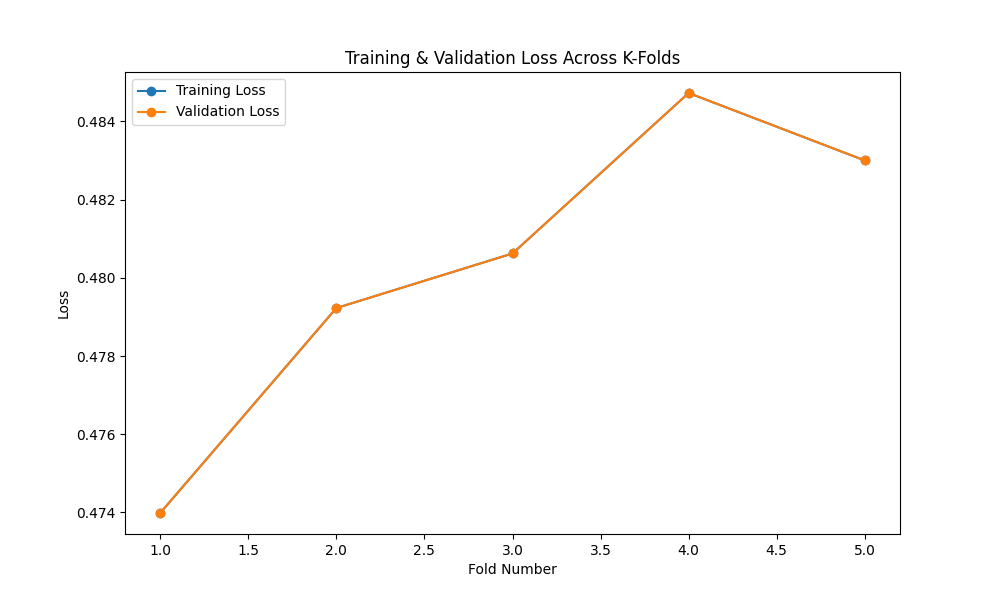
\includegraphics[width=\textwidth]{img/report_info/img/2.2.MLP/best_mlp_count_loss.png}
        \caption{Loss Curve - Count Vectorizer}
        \label{fig:mlp-count-loss}
    \end{subfigure}
    \begin{subfigure}[b]{0.44\textwidth}
        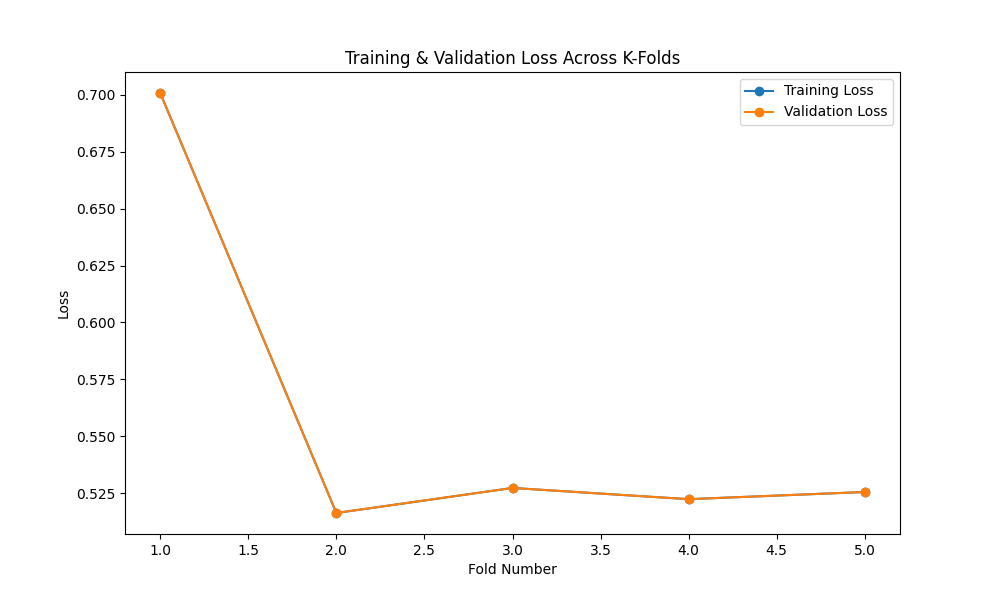
\includegraphics[width=\textwidth]{img/report_info/img/2.2.MLP/best_mlp_tfidf_loss.png}
        \caption{Loss Curve - TF-IDF}
        \label{fig:mlp-tfidf-loss}
    \end{subfigure}
    
    \begin{subfigure}[b]{0.44\textwidth}
        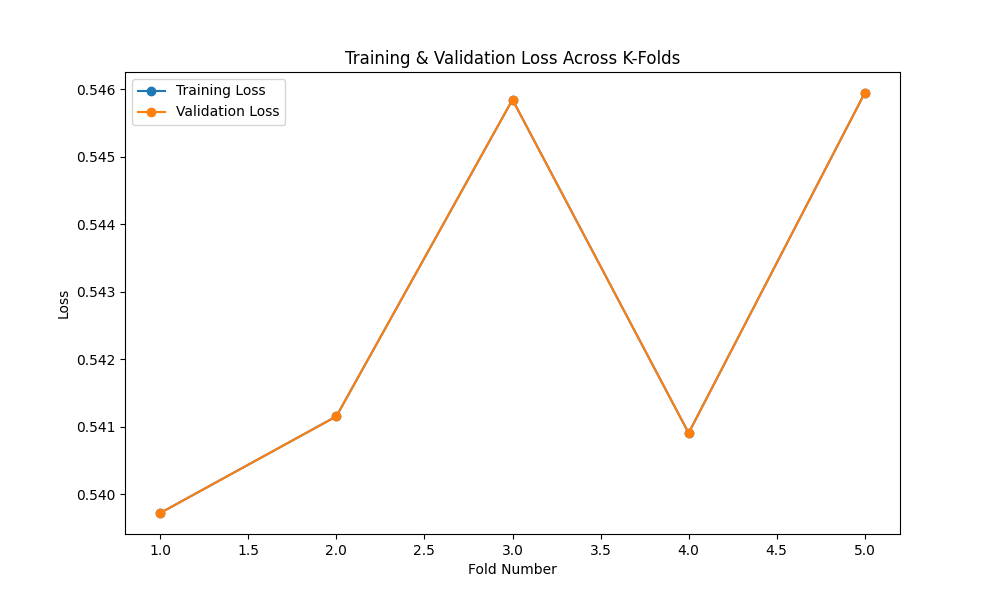
\includegraphics[width=\textwidth]{img/report_info/img/2.2.MLP/best_mlp_word2vec_loss.png}
        \caption{Loss Curve - Word2Vec}
        \label{fig:mlp-word2vec-loss}
    \end{subfigure}
    \begin{subfigure}[b]{0.44\textwidth}
        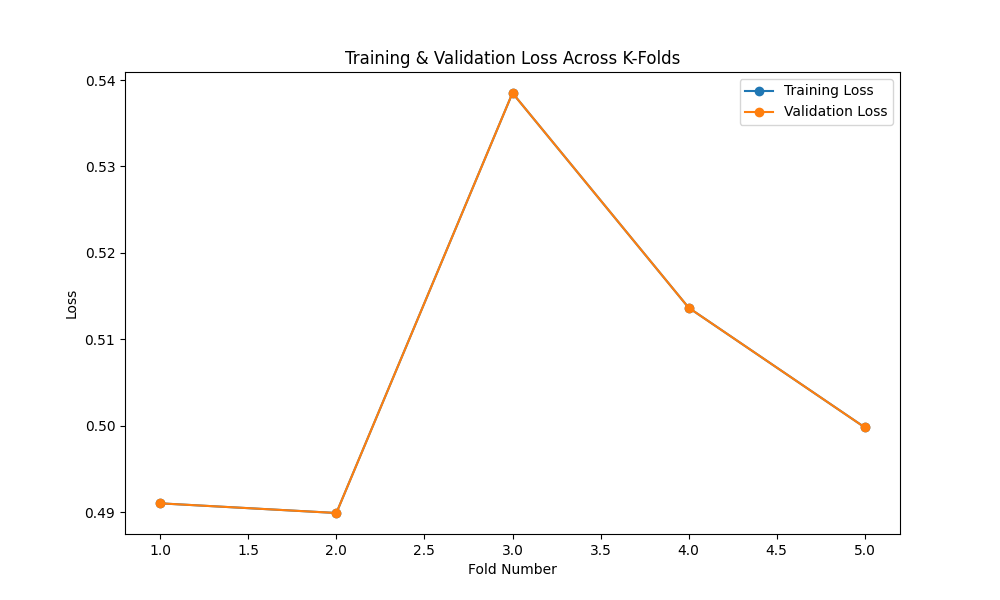
\includegraphics[width=\textwidth]{img/report_info/img/2.2.MLP/best_mlp_glove_loss.png}
        \caption{Loss Curve - GloVe}
        \label{fig:mlp-glove-loss}
    \end{subfigure}
    
    \caption{Comparison of Training and Validation Loss Curves for MLP across Different Feature Extraction Methods}
    \label{fig:mlp-loss-group}
\end{figure}

\begin{figure}[H]
    \centering
    \begin{subfigure}[b]{0.48\textwidth}
        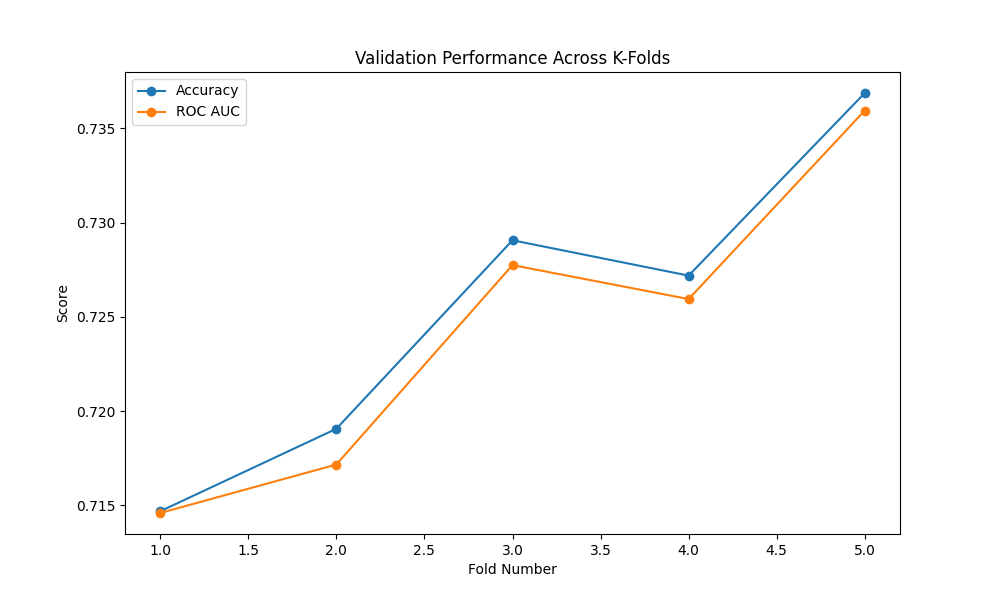
\includegraphics[width=\textwidth]{img/report_info/img/2.2.MLP/best_mlp_count.png}
        \caption{Performance - Count Vectorizer}
        \label{fig:mlp-count}
    \end{subfigure}
    \begin{subfigure}[b]{0.48\textwidth}
        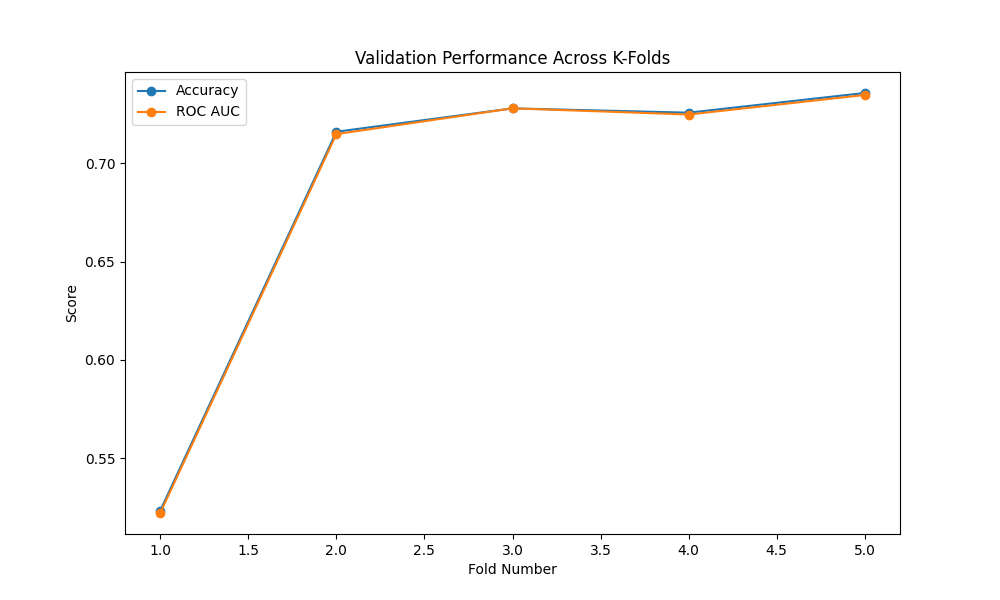
\includegraphics[width=\textwidth]{img/report_info/img/2.2.MLP/best_mlp_tfidf.png}
        \caption{Performance - TF-IDF}
        \label{fig:mlp-tfidf}
    \end{subfigure}
    
    \begin{subfigure}[b]{0.48\textwidth}
        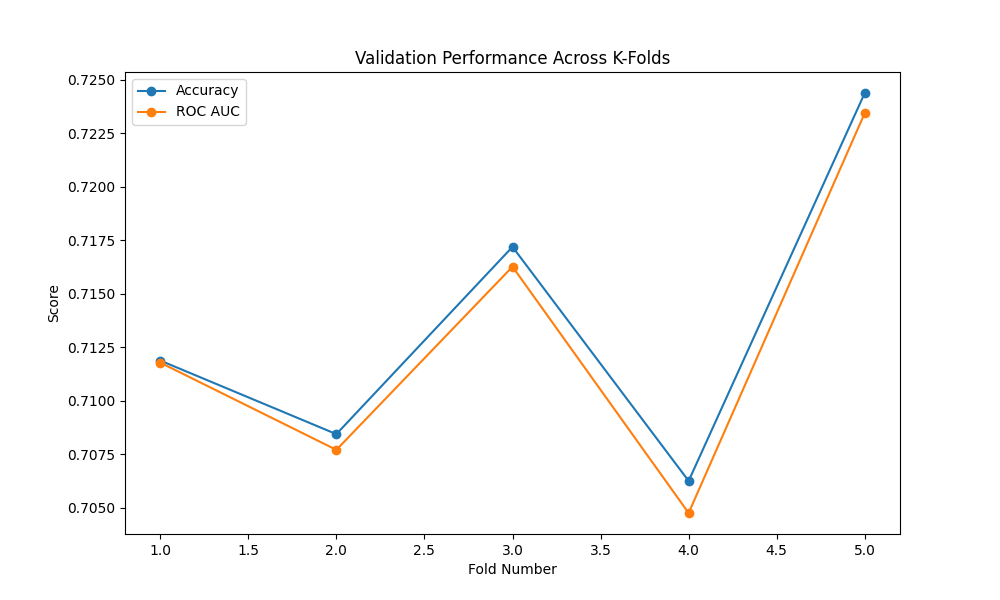
\includegraphics[width=\textwidth]{img/report_info/img/2.2.MLP/best_mlp_word2vec.png}
        \caption{Performance - Word2Vec}
        \label{fig:mlp-word2vec}
    \end{subfigure}
    \begin{subfigure}[b]{0.48\textwidth}
        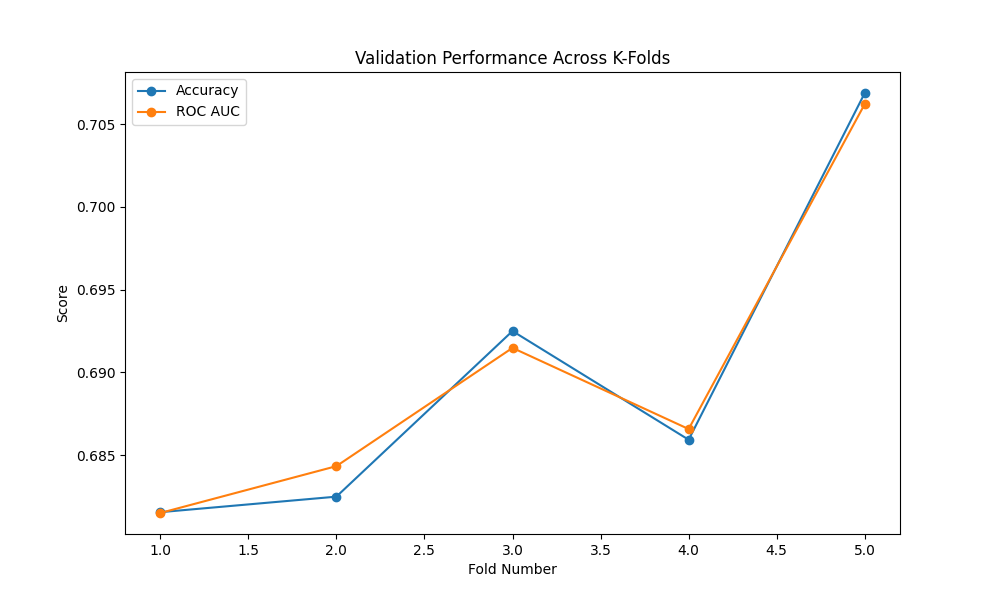
\includegraphics[width=\textwidth]{img/report_info/img/2.2.MLP/best_mlp_glove.png}
        \caption{Performance - GloVe}
        \label{fig:mlp-glove}
    \end{subfigure}
    
    \caption{Comparison of Training Performance Metrics for MLP across Different Feature Extraction Methods}
    \label{fig:mlp-performance-group}
\end{figure}

\textbf{Image Description:}

\begin{itemize}
    \item \textbf{Training and Validation Loss Analysis:}
    \begin{itemize}
        \item \textit{Count Vectorizer, TF-IDF}: Fairly stable validation loss across folds, with some minor increases in specific folds reflecting data shifts.
        \item \textit{Word2Vec, GloVe}: Show a bit more variance, suggesting the learned word embeddings can introduce additional complexity.
        \item Overall, the MLP’s training loss consistently decreases, indicating effective convergence via stochastic gradient descent.
    \end{itemize}
    
    \item \textbf{Validation Performance Metrics:}
    \begin{itemize}
        \item \textit{Accuracy}: Rises steadily for Count and TF-IDF, peaking around the later folds; Word2Vec and GloVe exhibit more fold-to-fold fluctuation.
        \item \textit{ROC AUC}: Mirrors accuracy trends; MLP achieves a decent margin between positive and negative classes for all embeddings.
        \item \textit{F1 Score}: High recall suggests MLP captures many true positives, while precision remains moderate across embeddings.
    \end{itemize}
\end{itemize}

These plots provide a clear visual indicator of how the MLP behaves with different text features. 
Count-based inputs tend to demonstrate smoother training curves and comparatively stronger 
validation scores, consistent with the numerical results reported in Table~\ref{tab:mlp-testing-metrics}.

\subsubsection{Conclusion}

The MLP model, despite its relatively simple design (a single hidden layer of 100 neurons), performs robustly across different text representations. Count Vectorization emerges as the top method in tandem with the MLP, achieving a 73.70\% accuracy and an F1 score of 0.7526. This highlights the strength of MLPs for classical bag-of-words features, as well as the effectiveness of appropriate hyperparameters and regularization.

Future enhancements might include:

\begin{itemize}
    \item Employing deeper MLP architectures or exploring \texttt{relu} activations.
    \item Incorporating batch normalization for faster, more stable convergence.
    \item Integrating pre-trained embeddings (e.g., GloVe or Word2Vec) in a more fine-tuned setup.
    \item Exploring advanced optimizers (e.g., \texttt{Adam}) for potentially better minima.
\end{itemize}

Overall, MLPs offer a solid, interpretable baseline that often competes well with more complex models, especially when dealing with moderate-sized datasets and straightforward text-based features.

